\section{Retransmission Response Packet Processing Module} 

The Retransmission Request Packet Processing module takes an input
retransmit request and attempts to acquire that packet. It then sends
that packet out to the interface. Note that the packet retrieved from
the FIFO may not be the packet requested, if the FIFO has since
wrapped around.

\subsection{Implementation}

A successful packet lookup results in the assertion of
\signal{RETXSUCCESS}. A failed look-up (in which we do not find a
packet with a completely-matching sequence ID) causes the assertion of
a \signal{PKTNOTINBUF}.


\begin{figure}
\begin{centering}
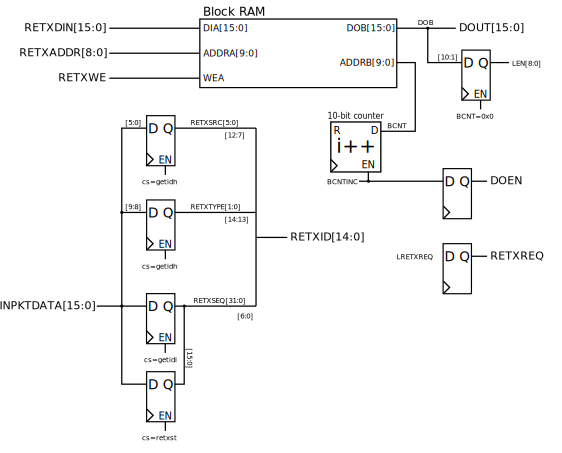
\includegraphics[scale=0.8]{retxresponse.svg}
\end{centering}
\caption{Retransmission Request module.}
\label{retxresponse}
\end{figure}

\begin{figure}
\begin{centering}
\includegraphics[scale=0.8]{retxresponse.fsm.svg}
\end{centering}
\caption{Retransmission Request module FSM.}
\label{retxresponse.fsm}
\end{figure}
